\subsection{Supervised learning}

One of the main types of automatic learning is supervised learning. This type of learning is akin to human learning based on the acquisition of new knowledge and skills through the experiences of the past. That means, the computer learns from data it has previously collected.

Changing the synaptic forces is based on the comparison between the output vector $ y ^ t = (y ^ t_1, y ^ t_2, ..., y ^ t_m), t = 1, ..., P $ obtained at the output layer and the target vector $ z ^ t = (z ^ t_1, z ^ t_2, ..., z ^ t_m), t = 1, ..., P $, representing the desired result to be obtained at the output layer, at the input layer the input vector $ x ^ t = (x ^ t_0, x ^ t_1, x ^ t_2, ..., x ^ t_n), t = 1, ..., P $ of the training.

The target vector $ z ^ t $ is provided by a teacher (coach-supervisor), hence the supervised learning name. Supervised learning involves the presentation by a coach of pairs of data form $ (x ^ t, z ^ t), t = 1, ..., P $ forming a set of data, called training set: $$ S = \{(x ^ t, z ^ t) | t = 1, ..., P \} $$

The difference between the obtained y response and the desired z response is the error and is used to modify the synaptic forces, based on a specific algorithm called \cite{calculNeuronal}.

We can represent supervised learning with the following diagram \cite{Baum}:

\begin{figure}[H]
  \centering
  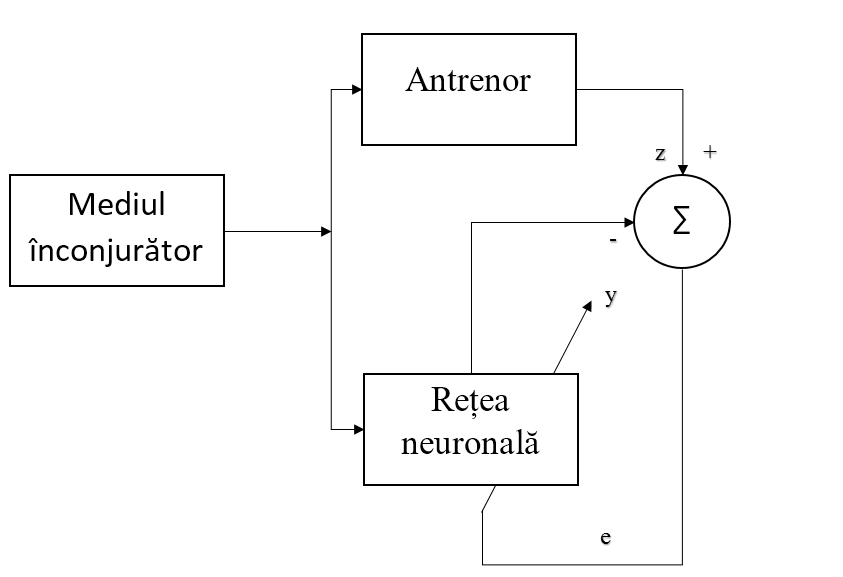
\includegraphics[width=3.5in]{images/diagramaInvSupervizate.png}
  \caption {Diagram of supervised learning.}
\end{figure}

It is seen from this diagram the equivalence of the supervised learning paradigm with the learning algorithm based on minimizing the error function \cite{Haykin}.